\section{Sequential Task Execution Experiment}
\label{sec:ex}
We conduct three experiments that include manipulations of large deformable objects:

\begin{enumerate}
  \item Wrapping an object with a cloth,
  \item Putting up a poster on a wall,
  \item Folding a table cloth.
\end{enumerate}

\figref{wrapping}, \figref{poster} and \figref{folding} show the vector fields of the environmental object and the snapshot in each experiment.

\section{Conclusions}
In this research, we proposed a method to achieve autonomous arm motion of robot in cooperative manipulation of large flexible objects. In our proposed method, the hand position following human hand movement and hand orientation considering positional relationship with environmental object are combined to derive robot arm motion. The effectiveness was demonstrated through experiments using the real robot HRP-2. %% The future task is to make our method applicable to rigid body operation and to integrate robot's other sensor information such as force sensor and to strengthen vision recognition when object geometry is unknown.

\vspace{-3mm}
\begin{figure}[htbp]
  \begin{minipage}{0.4\hsize}
    \begin{center}
      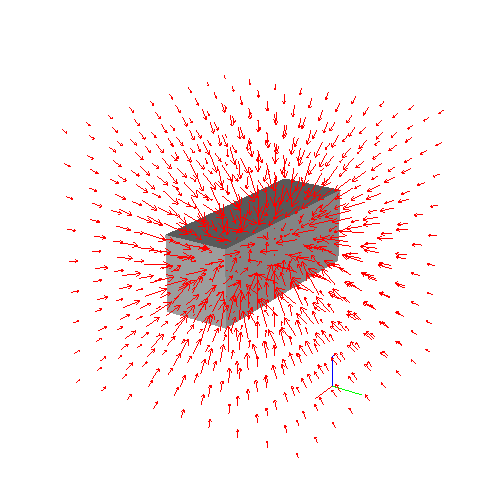
\includegraphics[width=1.00\columnwidth]{figs/electronic-potential-box-no-frame.png}
    \end{center}
  \end{minipage}
  \begin{minipage}{0.55\hsize}
    \begin{center}
      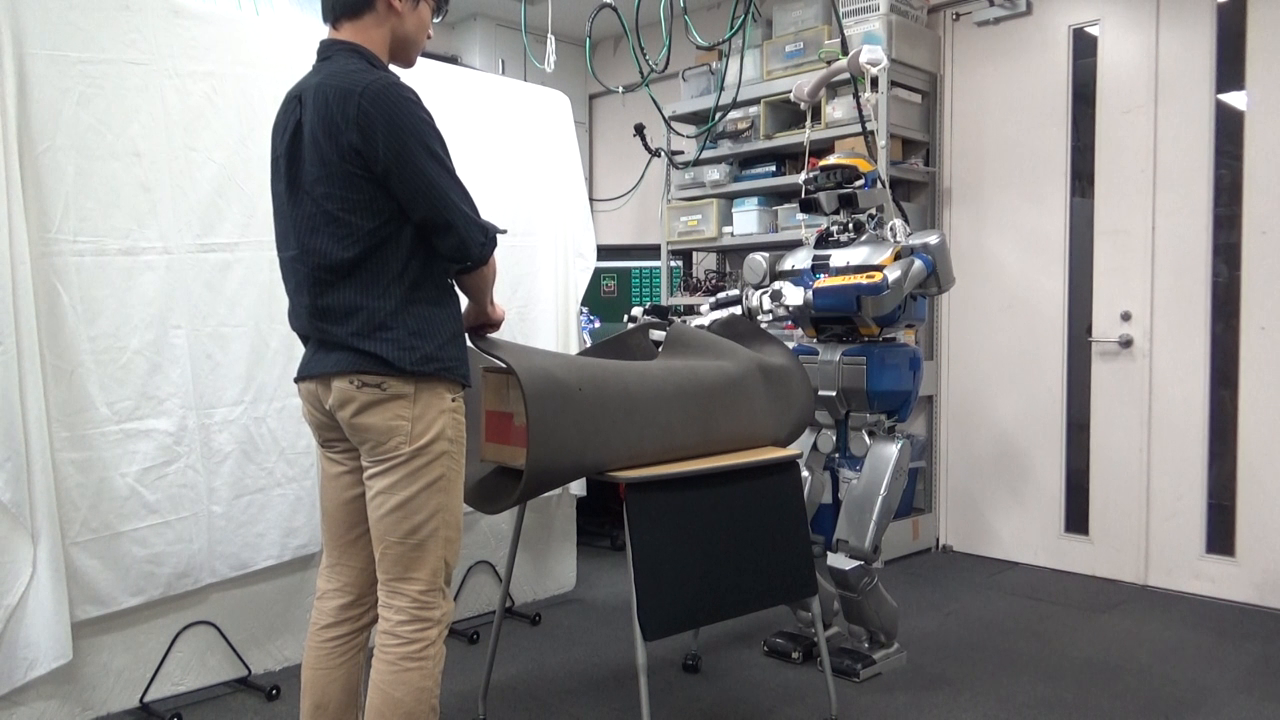
\includegraphics[width=1.00\columnwidth]{figs/image_wrap.png}
    \end{center}
  \end{minipage}
  \vspace{-3mm}
  \caption{Wrapping-box experiment}
  \label{figure:wrapping}
\end{figure}

\vspace{-8mm}
\begin{figure}[htbp]
  \begin{minipage}{0.4\hsize}
    \begin{center}
      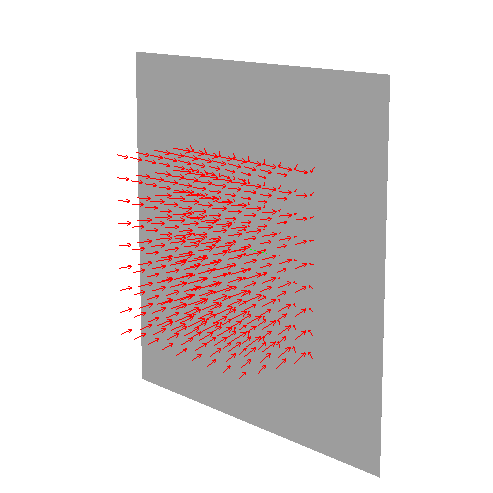
\includegraphics[width=0.90\columnwidth]{figs/electronic-potential-wall.png}
    \end{center}
  \end{minipage}
  \begin{minipage}{0.55\hsize}
    \begin{center}
      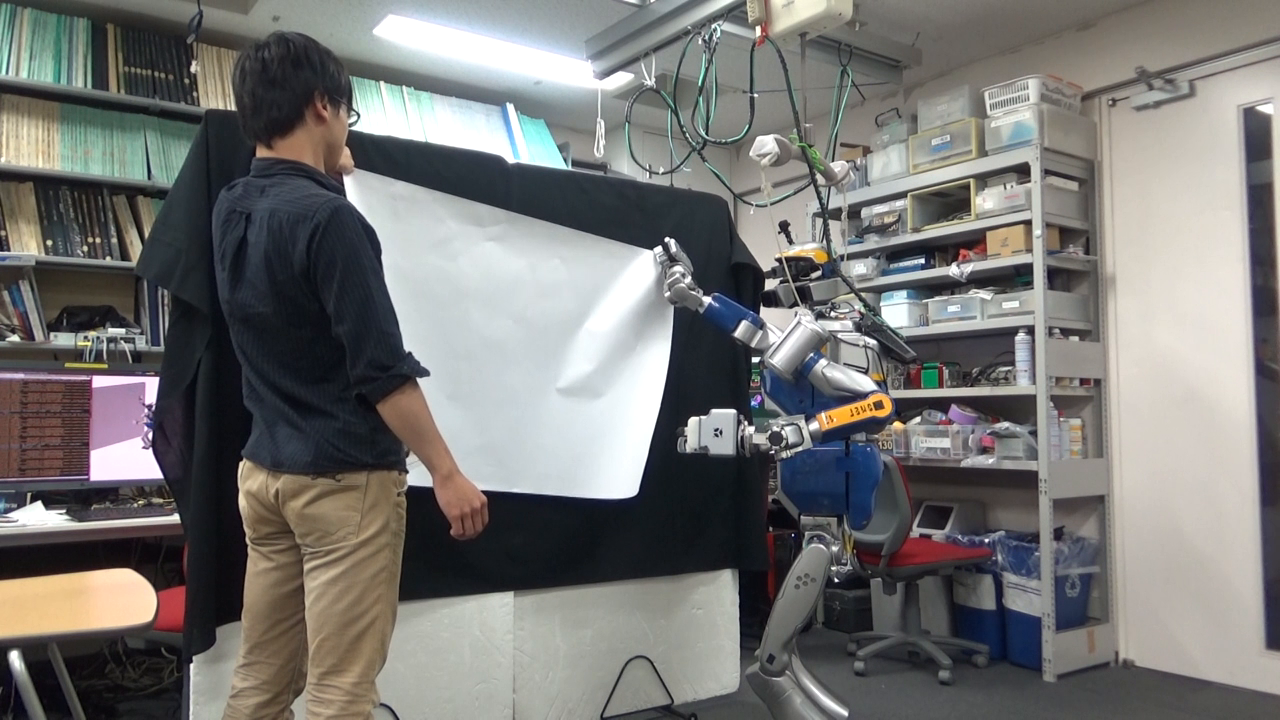
\includegraphics[width=1.00\columnwidth]{figs/image_poster.png}
    \end{center}
  \end{minipage}
  %% \vspace{-3mm}
  \caption{Putting-up-poster experiment}
  \label{figure:poster}
\end{figure}

\vspace{-5mm}
\begin{figure}[htbp]
  \begin{minipage}{0.4\hsize}
    \begin{center}
      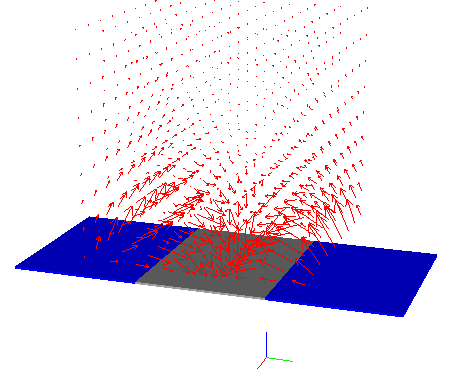
\includegraphics[width=1.00\columnwidth]{figs/electronic-potential-table-4.png}
    \end{center}
  \end{minipage}
  \begin{minipage}{0.55\hsize}
    \begin{center}
      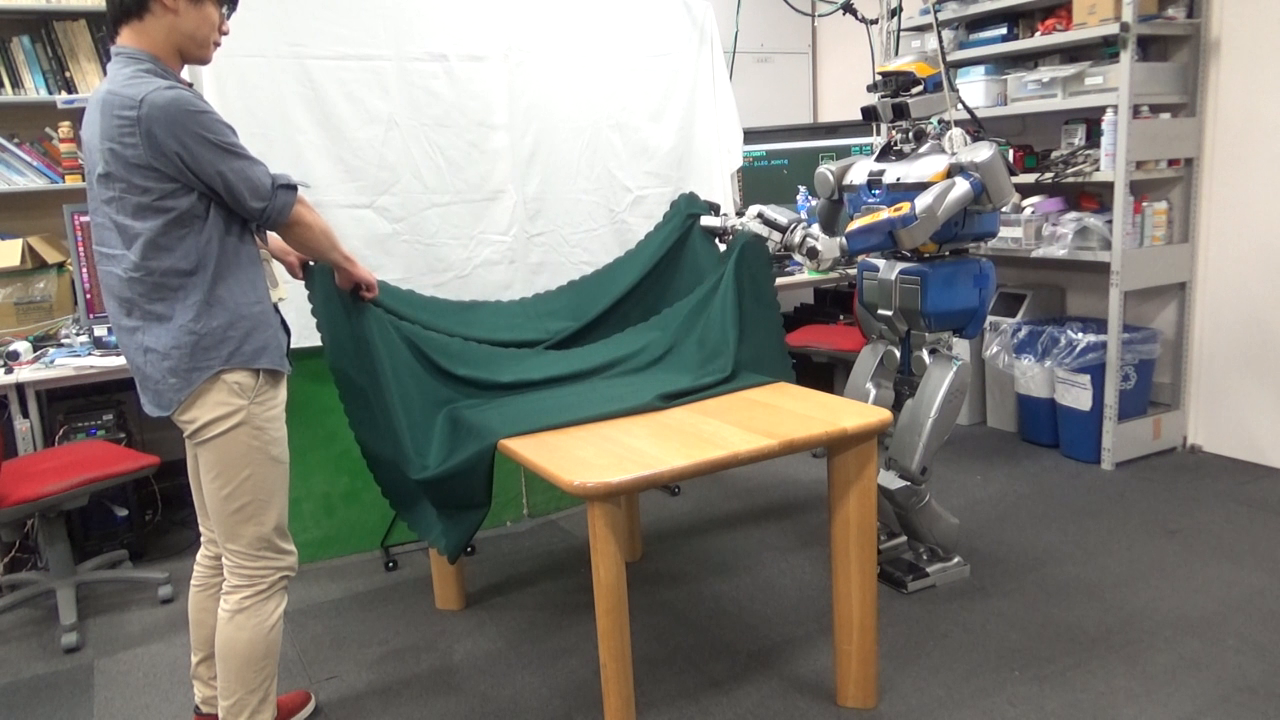
\includegraphics[width=1.00\columnwidth]{figs/image_fold.png}
    \end{center}
  \end{minipage}
  %% \vspace{-3mm}
  \caption{Folding-table-cloth experiment}
  \label{figure:folding}
\end{figure}
\vspace{-4mm}

